\documentclass{article}
\usepackage{svg}
\usepackage{hyperref}
\usepackage{amsmath}
\usepackage{amsfonts} 
\usepackage{graphicx}
\usepackage[a4paper,  total={6.75in, 10in}]{geometry}
\usepackage[utf8]{inputenc}


\title{swag di una pandemia con un modello SIRV}
\author{Giulio Pastorello }
\date{Ottobre 2023}

\begin{document}

\maketitle

\section{Il Modello}

\hspace{\parindent} Per descrivere l'andamento della pandemia si è scelto 
di usare un modello SIR al quale è stata aggiunta un quarta 
equazione per rappresentare i vaccinati.\\
Le equazioni che descrivono l'evoluzione della pandemia sono quindi:
\begin{itemize}
\item $S(t)$: "Susceptible". Descrive il numero delle persone non 
malate che non hanno mai contratto l'infezione.
\item $I(t)$: "Infected". Il numero di persone che ad un dato tempo 
t sono malate. 
\item $R(t)$: "Removed". Una volta che una persona è stata 
contagiata, dopo un certo intervallo di tempo viene \textit{rimossa}, 
ovvero guarisce o muore. Si assume che, una volta guariti, 
i soggetti diventino immuni. L'unica possibilità di transizione da 
uno stato all'altro è quindi: $S\xrightarrow{}I\xrightarrow{}R$.
\item $V(t)$: "Vaccinated". Questa equazione è un'aggiunta al modello 
SIR "standard", che prevede solo le prime tre equazioni. 
Anche in questo caso si fa l'assunzione che una persona vaccinata 
non possa più ammalarsi.
\end{itemize}
Il vincolo fondamentale del modello è che la popolazione totale 
sia costante:
\begin{equation}\label{eq::pop}
S(t)+I(t)+R(t)+V(t)=N
\end{equation}
Questa è un'approssimazione ragionevole se si fa l'assunzione 
che il numero totale di persone che muoiono a causa del virus 
sia trascurabile rispetto alla popolazione totale.
\subsection{Parametri}
Il modello descrive l'andamento della pandemia attraverso alcuni 
parametri:
\begin{itemize} 
\item $\beta \in [0,1]$: questo è interpretabile come la 
\textit{contagiosità} del virus, ovvero la probabilità di 
trasmissione a seguito di un contatto tra un suscettibile e un infetto.
\item $\gamma \in [0,1]$: è l'inverso della durata media di 
un'infezione, che corrisponde alla probabilità di guarigione o morte.
\item $\eta \in \mathbb{N}, \eta < N$: il numero di persone non 
vaccinabili, per motivi medici o personali.
\item $\mu \in\ [0,1]$: rappresenta la velocità delle vaccinazioni.
\item $\xi \in [0,1]$: rappresenta l'efficacia delle vaccinazioni. 
Si usa come fattore moltiplicativo.
\end{itemize}

\subsection{Condizioni Iniziali}
Per studiare la diffusione del virus vengono anche usati come 
condizioni iniziali i seguenti termini:
\begin{itemize}
\item $I_0 \in \mathbb{N}, I_0 < N$: malati al tempo $t = 0$.
\item $V_0 \in \mathbb{N}, V_0 < N $: vaccinati al tempo $t = 0$.
\item $R_0 \in \mathbb{N}, R_0 < N $: rimossi al tempo $t = 0$.
\end{itemize}
Ovviamente si avrà che il numero di suscettibili dall'inizio della 
simulazione ($t = 0$) $S_0$ sarà: \\
$S_0 = N - I_0 - V_0 - R_0$.\\
\subsection{Equazioni}
Usando i parametri descritti sopra, le equazioni differenziali che 
descrivono la diffusione della pandemia sono quindi quattro:\\
\begin{equation} \label{eq::S}
\frac{dS}{dt}(t)= -\beta \frac{S(t)}{N}I(t) - \frac{dV}{dt}(t)
\end{equation}
\begin{equation}\label{eq::I}
\frac{dI}{dt}(t)= \beta \frac{S(t)}{N}I(t) - \gamma I(t)
\end{equation}
\begin{equation}\label{eq::R}
\frac{dR}{dt}(t)= \gamma I(t)
\end{equation}
\begin{equation}\label{eq::V}
\frac{dV}{dt}(t)= \mu\frac{V(t)}{\xi}\left( 1-\frac{V(t)}{\xi(N-\eta)}\right)
\end{equation}
Una simulazione basata su dati rappresentativi dell'Emilia-Romagna
 è mostrata in figura (\ref{fig::SIRV}). 
 Si è usato: popolazione totale $N=4459000$, $\beta=0.05$, 
 $\gamma=0.02$, $I_0 = 530502$, $R_0 = 320000$, $V_0 = 600437$,
 non vaccinabili $\eta = 251042$, 
 velocità vaccinazioni $\mu = 0.05$, efficacia 
 vaccino $\xi= 0.83$.

 \subsection{Curva Logistica}
Per rappresentare la progressione della campagna vaccinale, 
nell'equazione (\ref{eq::V}) si è scelto di usare un'equazione 
logistica generalizzata: $f'(x)=f(x)(1-f(x))$,
che ha come soluzione un sigmoide. Quest'approssimazione è 
ragionevole perché ci si aspettava un inizio più lento dovuto alla 
scarsità di vaccini e all'organizzazione non ancora rodata, 
seguito da una crescita veloce della quantità di persone vaccinate, 
seguito inevitabilmente da una diminuzione dovuta al fatto che le 
persone da vaccinare sono sempre meno. 
Il limite dell'equazione logistica è che usando come numero di 
vaccinati iniziali $V_0  = 0$ la campagna vaccinale resta a zero, 
ma partendo da un qualsiasi altro numero si arriverà sicuramente a 
vaccinare tutti i vaccinabili, in un tempo che dipende dalla velocità 
delle vaccinazioni $\mu$. In figura (\ref{fig::vaccinati}) un 
andamento possibile della curva dei vaccinati.\\
\begin{figure}[h!]
\centering
\begin{minipage}[t]{.4\paperwidth}
    \hspace{-10pt}
    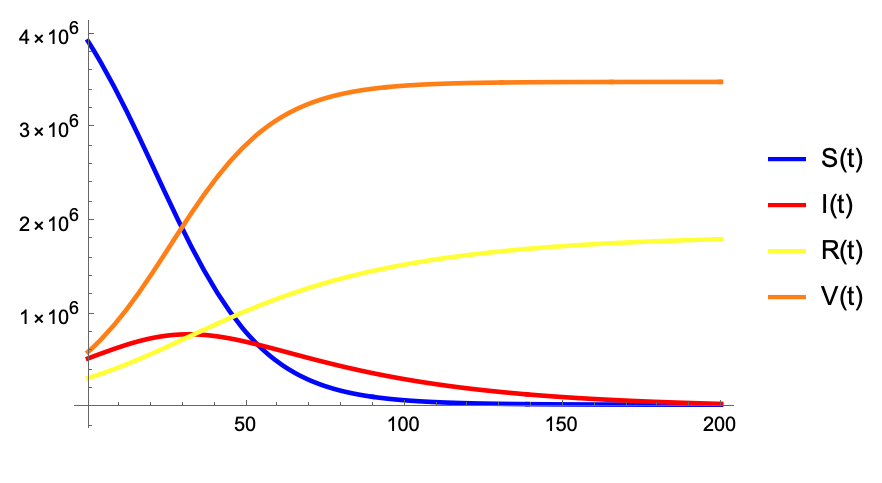
\includegraphics[width=\textwidth]{SIRV.png}
    \caption{\textit{Comportamento del modello SIRV con dati 
    rappresentativi dell'Emilia-Romagna}}
    \label{fig::SIRV}
    \end{minipage}%
\hfill %
\begin{minipage}[t]{.4\paperwidth}
    \hspace{-10pt}
    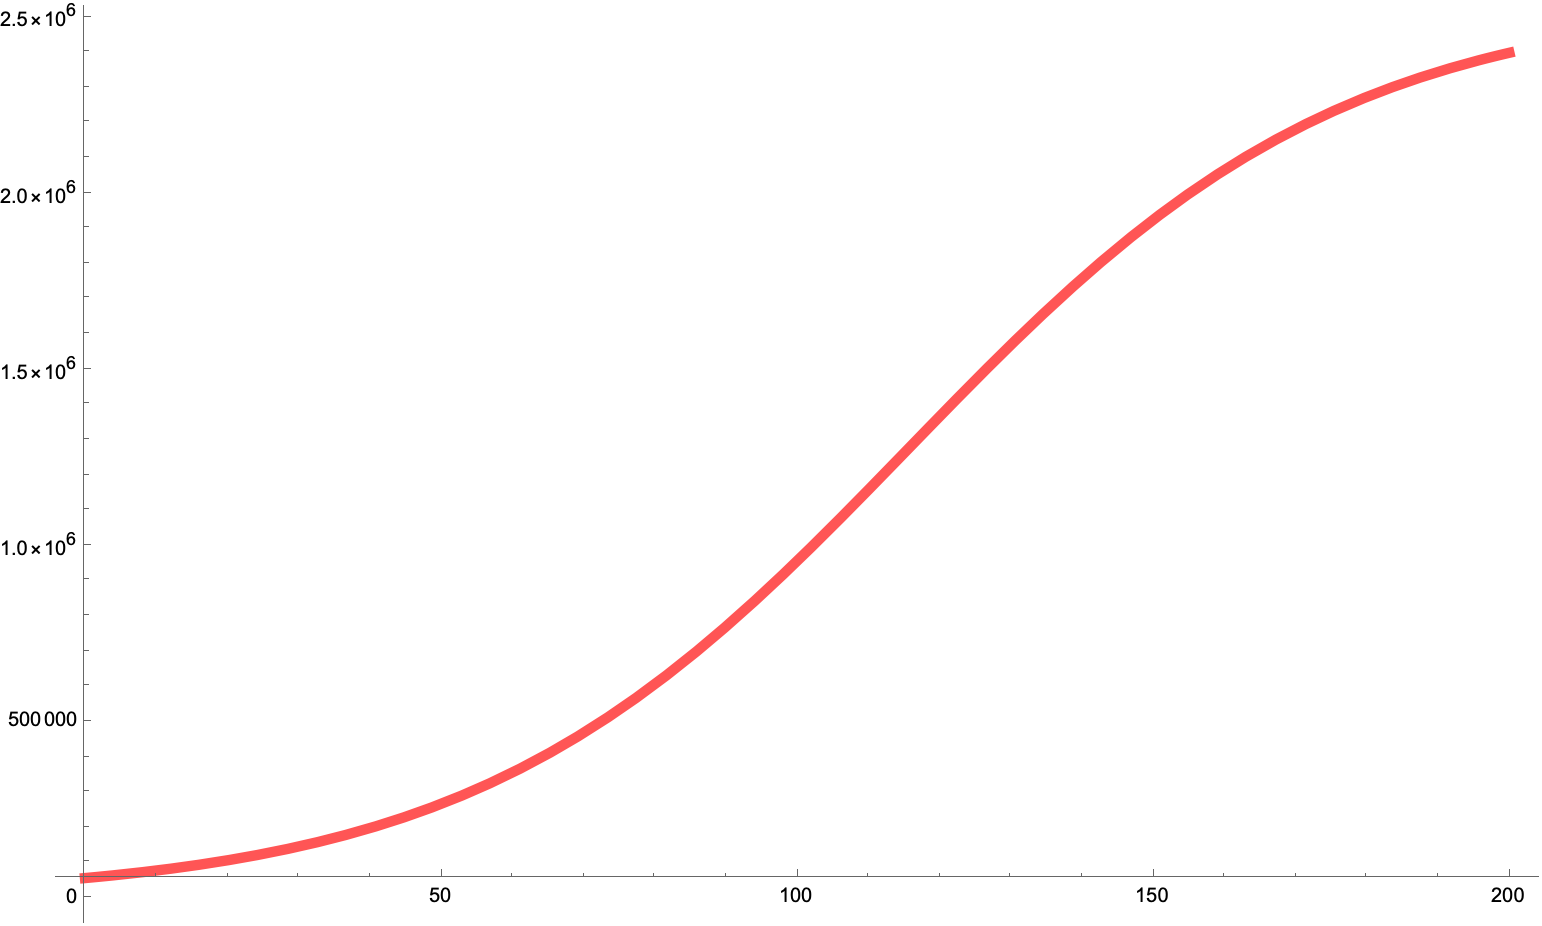
\includegraphics[width=\textwidth]{vaccinati.png}
    \caption{\textit{Curva logistica con $\nu=56980, 
    \mu=0.0274216, \eta=1418957$, e popolazione totale della regione 
    Emilia-Romagna.}}
    \label{fig::vaccinati}
\end{minipage}
\end{figure}

\section{I Metodi Numerici}

\hspace{\parindent} Per calcolare i risultati prodotti dal modello 
si sono scritti due diversi metodi numerici: il \textit{metodo di Eulero},
meno preciso ma anche meno dispendioso a livello di calcoli, e il 
metodo \textit{Runge-Kutta 4}, che è più complesso ma produce 
risultati migliori.

\subsection{Il metodo di Eulero}
Il metodo di Eulero è eseguito dalla funzione evolve() in 
infection.cpp. Dato un probelma di Cauchy nella forma
\begin{equation} \label{eq::ODE} 
    \dot{\vec{x}} = f(t, \vec{x}), \qquad \vec{x}(t_0) = \vec{x_0}
\end{equation}
dove $f(t, \vec{x})$ rappresenta il campo vettoriale che descrive il 
sistema di equazioni, con $\vec{x} \in \mathbb{R}^n$ variabile di stato, 
t variabile indipendente (tempo), e $\vec{x}(t_0) = \vec{x_0}$
condizione iniziale, il \textit{metodo di Eulero} discretizza il 
sistema nella seguente maniera:
\begin{equation} \label{eq::Euler}
    \vec{x}(t_{n+1})=\vec{x}(t_n) + h f(t_n, \vec{x}(t_n))
\end{equation}
dove h è lo \textit{step size}, un intervallo di tempo arbitrario che 
ovviamente determina la precisione dei risultati ottenuti. 
Nel caso dell'\textit{algoritmo di Eulero}, si dimostra che l'errore 
totale è dell'ordine di $O(h^2)$. \\
Nel caso del modello SMRV, il sistema è \textit{autonomo}, ovvero le 
euqazioni non dipendono esplicitamente dal tempo. L'algoritmo di 
discretizzazione assume quindi la forma: 
\begin{equation} \label{eq::autoEuler}
    \vec{x}(t_{n+1})=\vec{x}(t_n) + h f(\vec{x}(t_n))
\end{equation}
Le equazioni risultanti sono i valori che stampiamo:
\begin{equation}\label{eq::evolve}
    \left\{ \arraycolsep=1.4pt\def\arraystretch{2.2}
    \begin{array}{rcl}
    S(t_{n+1}) & = & S(t_n) + h \left(-\beta \frac{S(t_n)}{N} I(t_n)
            - \mu \frac{V(t_n)}{\xi} \left(
            1 - \frac{V(t_n)}{\xi (N - \eta)} \right) \right) \\
    M(t_{n+1}) & = & M(t_n)+h\left(\beta \frac{S(t_n)}{N} I(t_n) 
            - \gamma M(t_n)\right) \\
    R(t_{n+1}) & = & R(t_n) + h \gamma M(t_n) \\
    V(t_{n+1}) & = & V(t_n) +h \mu \frac{V(t_n)}{\xi} \left(
            1 - \frac{V(t_n)}{\xi (N - \eta)} \right) \\
    \end{array}\right.
\end{equation}
Sfruttando il vincolo della popolazione totale costante espresso 
dall'eq. (\ref{eq::pop}), si può "rimuovere una delle quattro 
equazioni esprimendone il valore in funzione delle altre tre.
Il risultato che otteniamo è il seguente:
\begin{equation}\label{eq::ezEvolve}
    \left\{ \arraycolsep=1.4pt\def\arraystretch{2.2}
    \begin{array}{rcl}
    V(t_{n+1}) & = & V(t_n) +h \mu \frac{V(t_n)}{\xi} \left(
        1 - \frac{V(t_n)}{\xi (N - \eta)} \right) \\
    S(t_{n+1}) & = & S(t_n) + h \left(-\beta \frac{S(t_n)}{N} I(t_n)
        - \Delta V \right) \\
    R(t_{n+1}) & = & R(t_n) + h \gamma M(t_n) \\
    M(t_{n+1}) & = & M(t_n) + h \left(-\Delta V - \Delta S - 
        \Delta R\right) \\
    \end{array}\right.
\end{equation}
dove si è usata la notazione $\Delta X = X(t_{n+1})-X(t_n)$. Questo
permette di ridurre il numero di valori da calcolare per ogni 
iterazione da 4 a 3.

\subsection{Runge-Kutta 4th Order}
L'algoritmo alternativo usato per calcolare i valori delle variabili di 
stato giorno-per-giorno è il Runge-Kutta del quarto ordine, abbreviato 
spesso come RK o RK4, che è eseguito nella funzione rk() in rk.cpp.
Come da nome, l'errore totale è dell'ordine di $O(h^4)$.
Partendo da un'equazione generica nella forma dell' eq. (\ref{eq::ODE})
l'approssimazione che viene fatta è la seguente: \\
\begin{equation} \label{eq::rk4}
    \vec{x}(t_{n+1})=\vec{x}(t_n)+\frac{h}{6}(k_1+k_2+k_3+k_4), \qquad
    \left\{ \arraycolsep=1.4pt\def\arraystretch{2.2}
    \begin{array}{rcl}
    k_1 & = & f(t_n, \vec{x}(t_n)) \\
    k_2 & = & f(t_n+\frac{h}{2}, \vec{x}(t_n)+h\frac{k_1}{2}) \\
    k_3 & = & f(t_n+\frac{h}{2}, \vec{x}(t_n)+h\frac{k_2}{2}) \\
    k_4 & = & f(t_n+h, \vec{x}(t_n)+hk_3) \\
    \end{array}\right.
\end{equation}
Nel caso del nostro modello, ricordando che il sistema è autonomo (ovvero
il campo è nella forma $f(\vec{x})$), il calcolo dei coefficienti è dato 
dalle seguenti espressioni:
\begin{equation} \label{eq::rk4Coeff}
    \left\{ \arraycolsep=1.4pt\def\arraystretch{2.2}
    \begin{array}{crcl}
    (V) & a_1 & = & \mu \frac{V(t)}{\xi}\left(1-\frac{V(t)}
    {\xi(N-\eta)}\right) \\
    (S) & b_1 & = &  -\beta\frac{S(t)}{N}M(t)-a_1\\
    (R) & c_1 & = &  \gamma M(t)\\
    (M) & d_1 & = &  -a_1-b_1-c_1 \\
    \end{array}\right. \quad
    \left\{ \arraycolsep=1.4pt\def\arraystretch{2.2}
    \begin{array}{rcl}
    a_2 & = & \mu \frac{V(t) + a_1 h/2}{\xi}\left(1-\frac{V(t)+
    a_1 h/2}{\xi(N-\eta)}\right) \\
    b_2 & = &  -\beta\frac{S(t)+b_1 h/2}{N}(M(t)+d_1 h/2)-a_2\\
    c_2 & = &  \gamma (M(t)+d_1 h/2)\\
    d_2 & = &  -a_2-b_2-c_2 \\
    \end{array}\right. \quad ...
\end{equation}
Scegliendo lo step size $h=1$(giorno), si otterranno i valori delle 
quattro variabili di ogni giorno. Ad ogni iterazione vengono ri-calcolati
i coefficienti $a_i, b_i, c_i,d_i, i \in \{1,2,3,4\}$, che sarebbero dunque
16 valori per ogni giornata. Usando lo stesso ragionamento di prima sul 
vincolo, si riesce a esprimere uno dei quattro coefficienti in funzione 
degli altri  tre, e quindi i valori da calcolare si riducono a 12 per ogni 
giornata.\\
\end{document}
